The convolutional layers are what makes CNN's such a strong tool. In general, a convolution consists of a set of learnable filters. Applying a convolutional operation on a neuron is done by using these filters to transform the input in some way, and output the transformed data. As mentioned earlier, CNNs can detect important patterns. The detections of these patterns are happening in these convolutional operations.\\

\noindent
These filters also called 'kernels', are simply just small matrixes initialized with some predefined dimensions and random values. When a kernel is applied on some feature map, the kernel simply convolve across all the feature-channels.\\

\noindent
Having a $M$x$M$ kernel $g$ with stride $1$x$1$, will take the center of the kernel, and stride the kernel over all possible regions of the input, where the kernel can fit. Simply finding the dot-product between the regional values of the input $f$, and the kernel values of $g$.

$$ g = \begin{bmatrix}
1/9 & 1/9 & 1/9 \\
1/9 & 1/9 & 1/9 \\
1/9 & 1/9 & 1/9
\end{bmatrix}
$$

\noindent
This means, that if some were to use, the filter kernel g, on some input feature map. This filter g would simply be a mean filter for the input; averaging all input regions. thus the output features will consist of a matrix with values of all the regions averaged. Using a filter greater than $1$x$1$ will yield a smaller output matrix.

\begin{figure}[!ht]
  \centering
  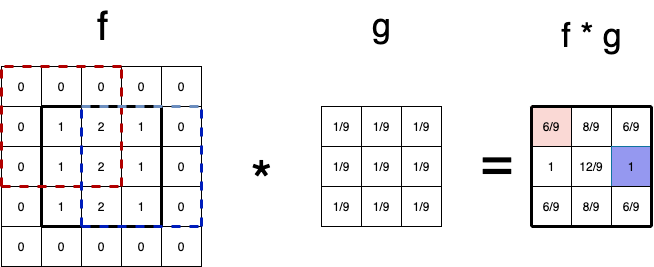
\includegraphics[scale=0.4]{latex/IMGs/conv1.png}
  \caption{Shows how a 3x3 mean filter acts on a 5x5 pixel feature map, with stride 1x1}\label{Baseline:before}
\end{figure}

\noindent
Given that we are looking at sequences, which are not two dimensional, but one dimensional, the filtering will look like:

\begin{figure}[!ht]
  \centering
  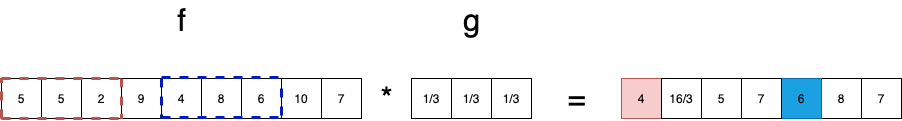
\includegraphics[scale=0.4]{latex/IMGs/conv2.png}
  \caption{Shows how a 1x3 mean filter acts on a 1x9 feature map, with stride 1}\label{Baseline:before}
\end{figure}

\noindent
Lastly, the convolutional layers have something called stride. The stride value defines how the filter travels over the input. Meaning how many steps it takes before calculating a new dot-product. In the example given above, we have a stride size of $1$x$1$. This means, that every single region where a $3$x$3$ can fit in the input, the dot-product will be calculated. If we were to change the stride to size $2$x$1$, the output would become smaller, since we take bigger steps, before taking the dot-product.

\begin{figure}[!ht]
  \centering
  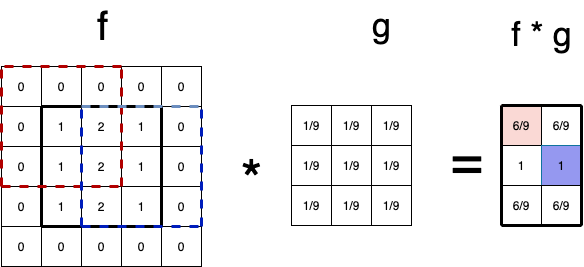
\includegraphics[scale=0.4]{latex/IMGs/conv1_stride.png}
  \caption{Shows how a 3x3 mean filter acts on a 5x5 pixel feature map, with stride 2x1}\label{Baseline:before}
\end{figure}

\begin{figure}[!ht]
  \centering
  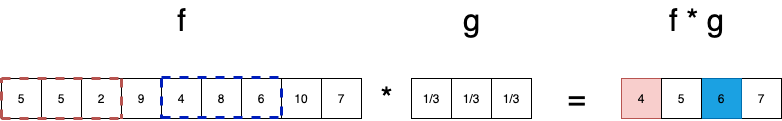
\includegraphics[scale=0.4]{latex/IMGs/conv2_stride.png}
  \caption{Shows how a 1x3 mean filter acts on a 1x9 feature map, with stride 2}\label{Baseline:before}
\end{figure}


